\section{Шина I2C}

\subsubsection{Устройство шины I2C}

I2C [\ref{i2c_protocol_spec}] — последовательная шина данных для связи интегральных схем, использующая две двунаправленные линии связи. Используется для соединения низкоскоростных периферийных компонентов с материнской платой, встраиваемыми системами и мобильными телефонами. Название представляет собой аббревиатуру слов Inter-Integrated Circuit. Шина данных поддерживает ``горячее'' подключение устройств (без перезапуска всей системы), а также одновременную работу нескольких ведущих устройств.

Данные передаются по двум проводам — \textit{линии данных} (SDA) и \textit{линии тактов} (SCL). В обмене всегда участвует два устройства: ведущий (\textit{master}) и ведомый (\textit{slave}). Тактовый сигнал на линии SCL генерируется ведущим устройством; ведомое устройство использует этот сигнал как опорный в том числе и для передачи данных к ведущему. Всего на одной двупроводной шине может быть до 127 устройств (адрес ведомого устройства кодируется 7 битами данных).

Каждая линия подключена к ``плюсу'' питания устройства через специальный \textit{подтягивающий резистор}. Таким образом, когда шина свободна  (обмены не производятся), с обеих линий считывается высокий уровень напряжения (логическая единица). Когда устройство начинает передачу, оно подключает требуемую линию к ``минусу'' питания и на линии устанавливается низкий уровень напряжения (логический ноль). Такая схема подключения называется \textit{монтажное ``И''}. Она позволяет нескольким устройствам устанавливать уровни одновременно без риска образования короткого замыкания и, как следствие, повреждения устройств.

Обмен начинается с события \textbf{START}, когда ведущее устройство устанавливает низкий уровень на линии данных (SDA) при высоком уровне на линии тактирования (SCL). В этот момент остальные устройства на линии определяют шину как занятую и ожидают окончания передачи.

После события \textbf{START} ведущее устройство передаёт байт, содержащий адрес ведомого устройства (7 бит) и бит режим обмена: 1 (R) - получение данных от ведомого устройства (чтение), 0 (W) - передача данных ведомому устройству (запись). Если на линии есть устройство с указанным адресом, оно должно установить линию SDA в низкий уровень для подтверждения приёма (событие \textbf{ACK}, от англ. acknowledge - подтверждение).

После этого происходит непосредственно обмен данными: в зависимости от выбранного режима, либо данные передаются от ведомого устройства, либо от ведущего. Получатель должен подтверждать приём каждого байта (исключение делается только для последнего байта в режиме чтения данных - master должен сообщить ведомому устройству об окончании приёма). Тактовый сигнал генерируется ведущим устройством, но при необходимости ведомое устройство может устанавливать тактовую линию в низкий уровень и, таким образом, задерживать обмен (например, если не успевает обрабатывать данные).

В конце обмена ведущее устройство меняет состояние линии SDA с низкого на высокий при высоком уровне на линии SCL - событие \textbf{STOP}. После этого шина считается освобождённой и в ней могут начинаться новые обмены. Стандарт I2C допускает также начало нового обмена тем же ведущим устройством, которое вело предыдущий обмен, без освобождения линии (если между обменами нет значительной паузы) - так называемое событие ``повторный START''.

\begin{figure}[H]
 \centering
 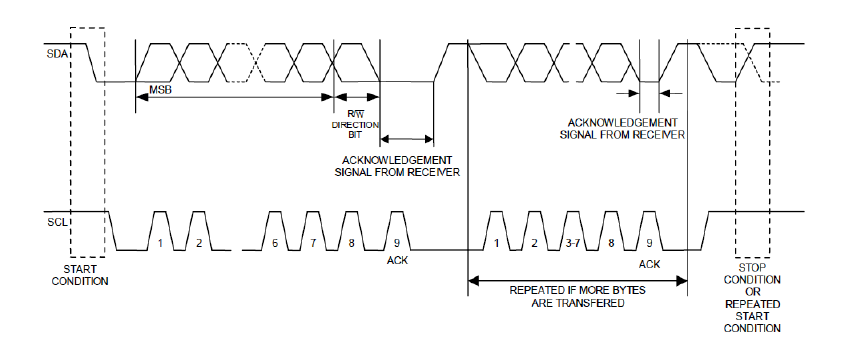
\includegraphics[width=\textwidth]{i2c_exchange}
 \caption{Структура информационного обмена на шине I2C}
 \label{fig:i2c_exchange}
\end{figure}

Таким образом, \textbf{обменом} на шине I2C будем считать последовательность управляющих сигналов и данных, которая начинается с события \textbf{START} и заканчивается событием \textbf{STOP} или \textbf{START}.

Обмен может содержать ошибки. Следующие ошибки могут быть обнаружены на этапе считывания обмена:

\begin{itemize}
 \item ведомое устройство не найдено - отсутствует ACK после первого байта обмена;
 \item ведомое устройство потеряно или неисправно - отсутствует ACK после переданного байта;
 \item некорректное начало передачи - отсутствует событие \textbf{START}.
\end{itemize}


Для представления корректного обмена нужно отобразить следующую информацию:

\begin{itemize}
 \item \textbf{время начала обмена} - время возникновения события \textbf{START};
 \item \textbf{длительность обмена} - время между событиями \textbf{START} и \textbf{STOP} (или повторным \textbf{START};
 \item адрес ведомого устройства;
 \item режим передачи - R или W;
 \item передаваемые данные (полезная нагрузка, payload).
\end{itemize}